\begin{figure}[h!]
\centering
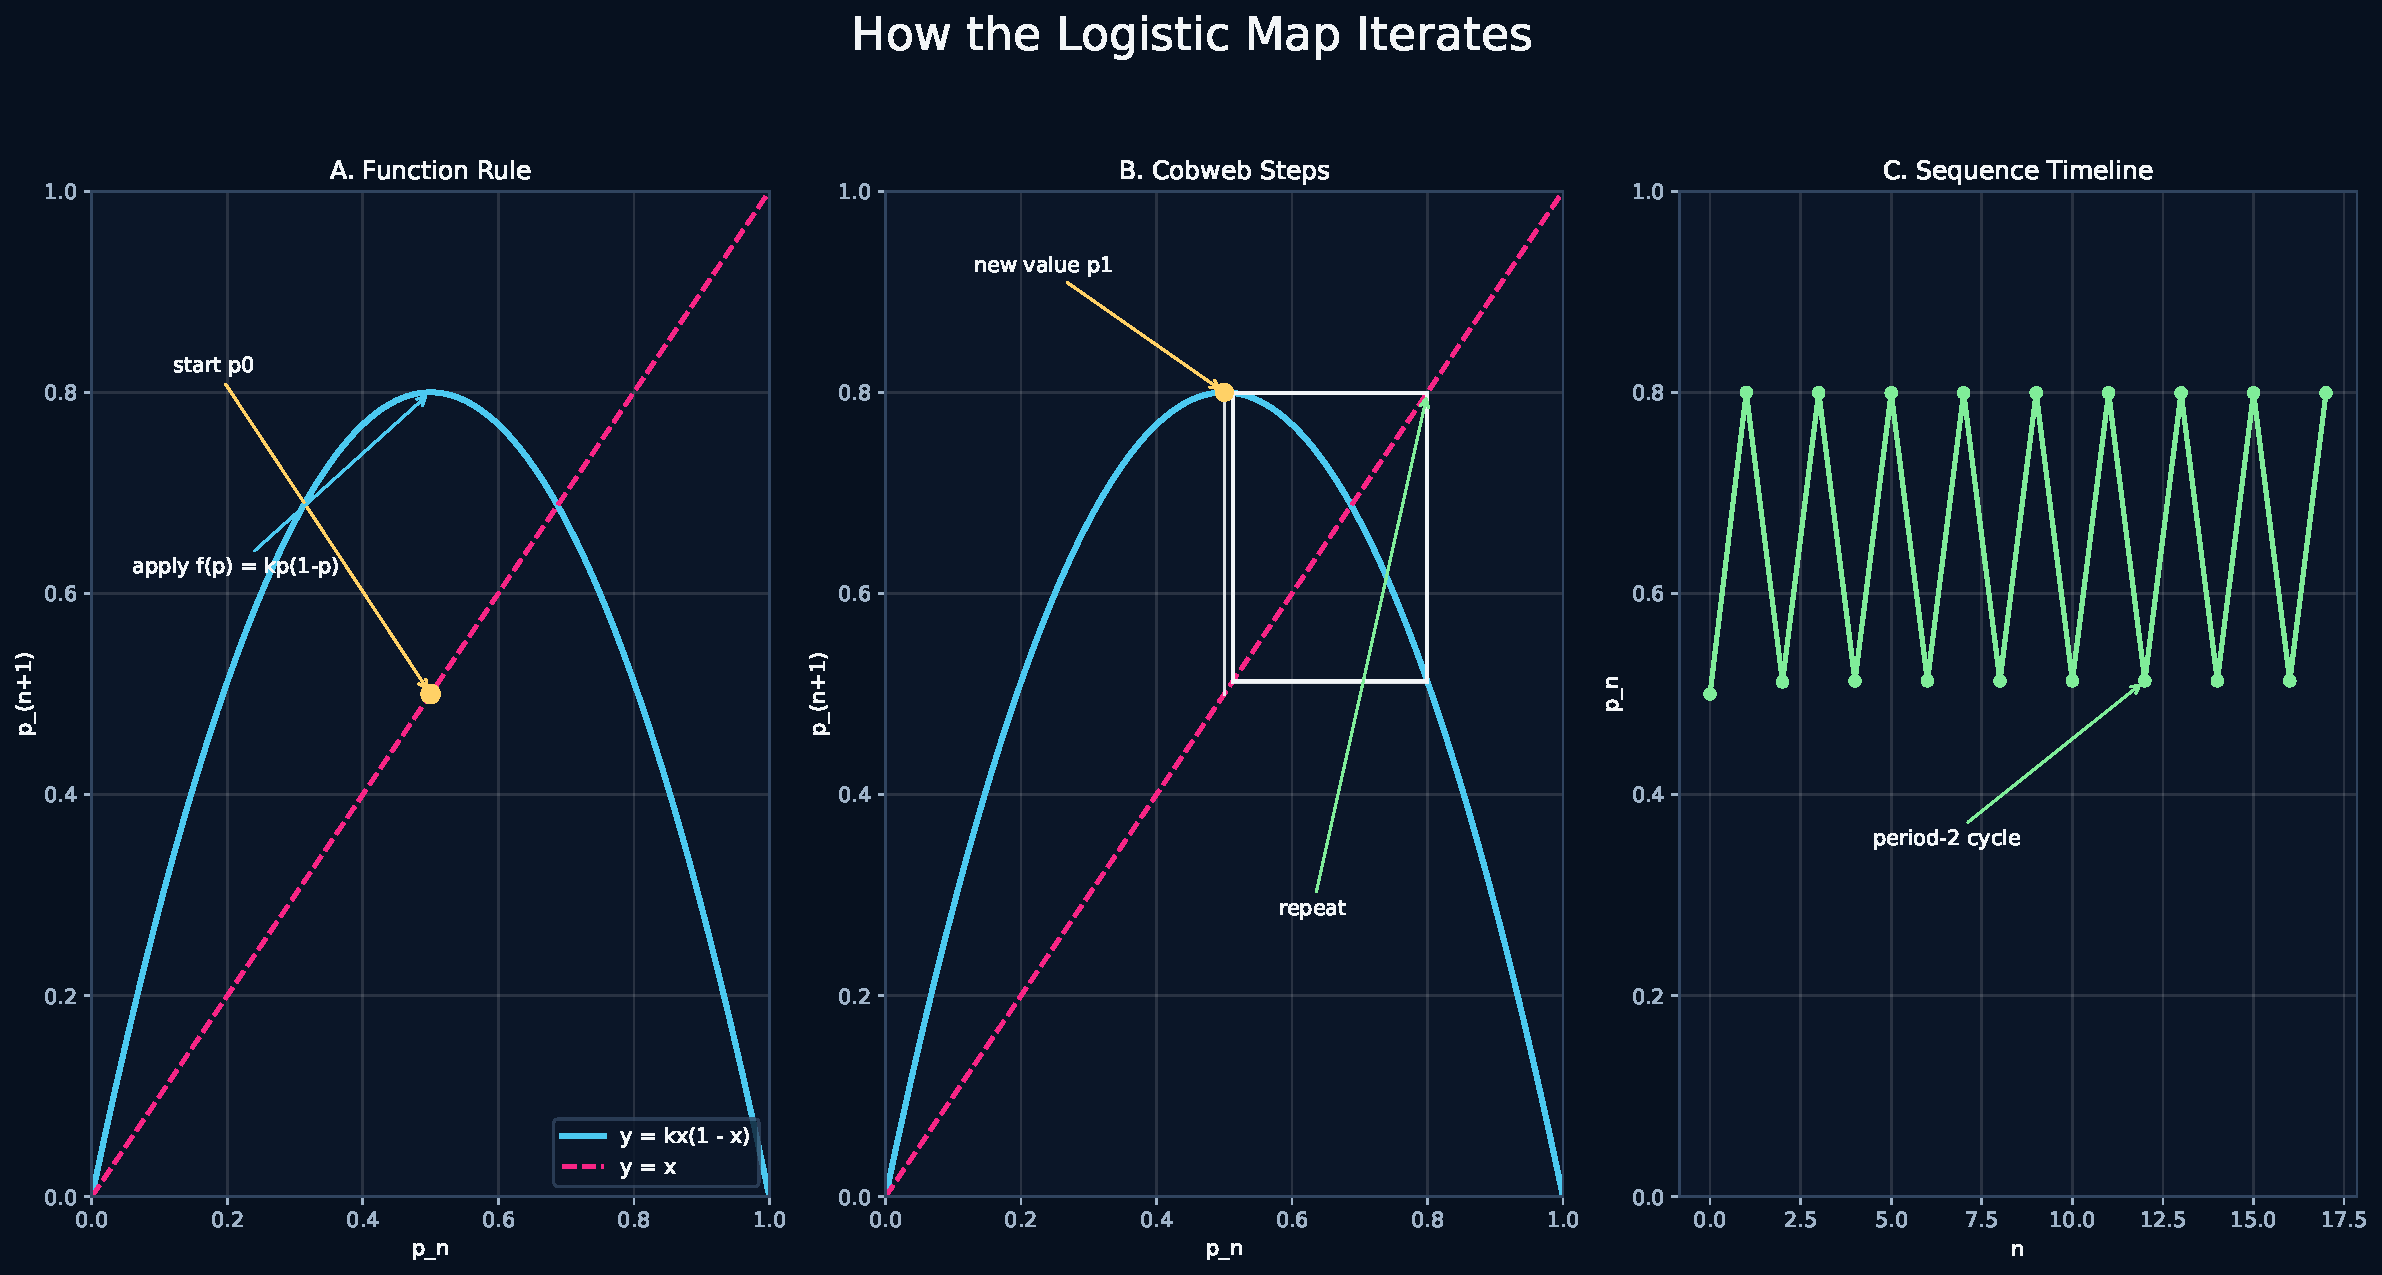
\includegraphics[width=\textwidth]{presentation_graphs/process_map.pdf}
\caption{How the logistic map produces each new value from the previous value.}
\end{figure}

\begin{figure}[h!]
\centering
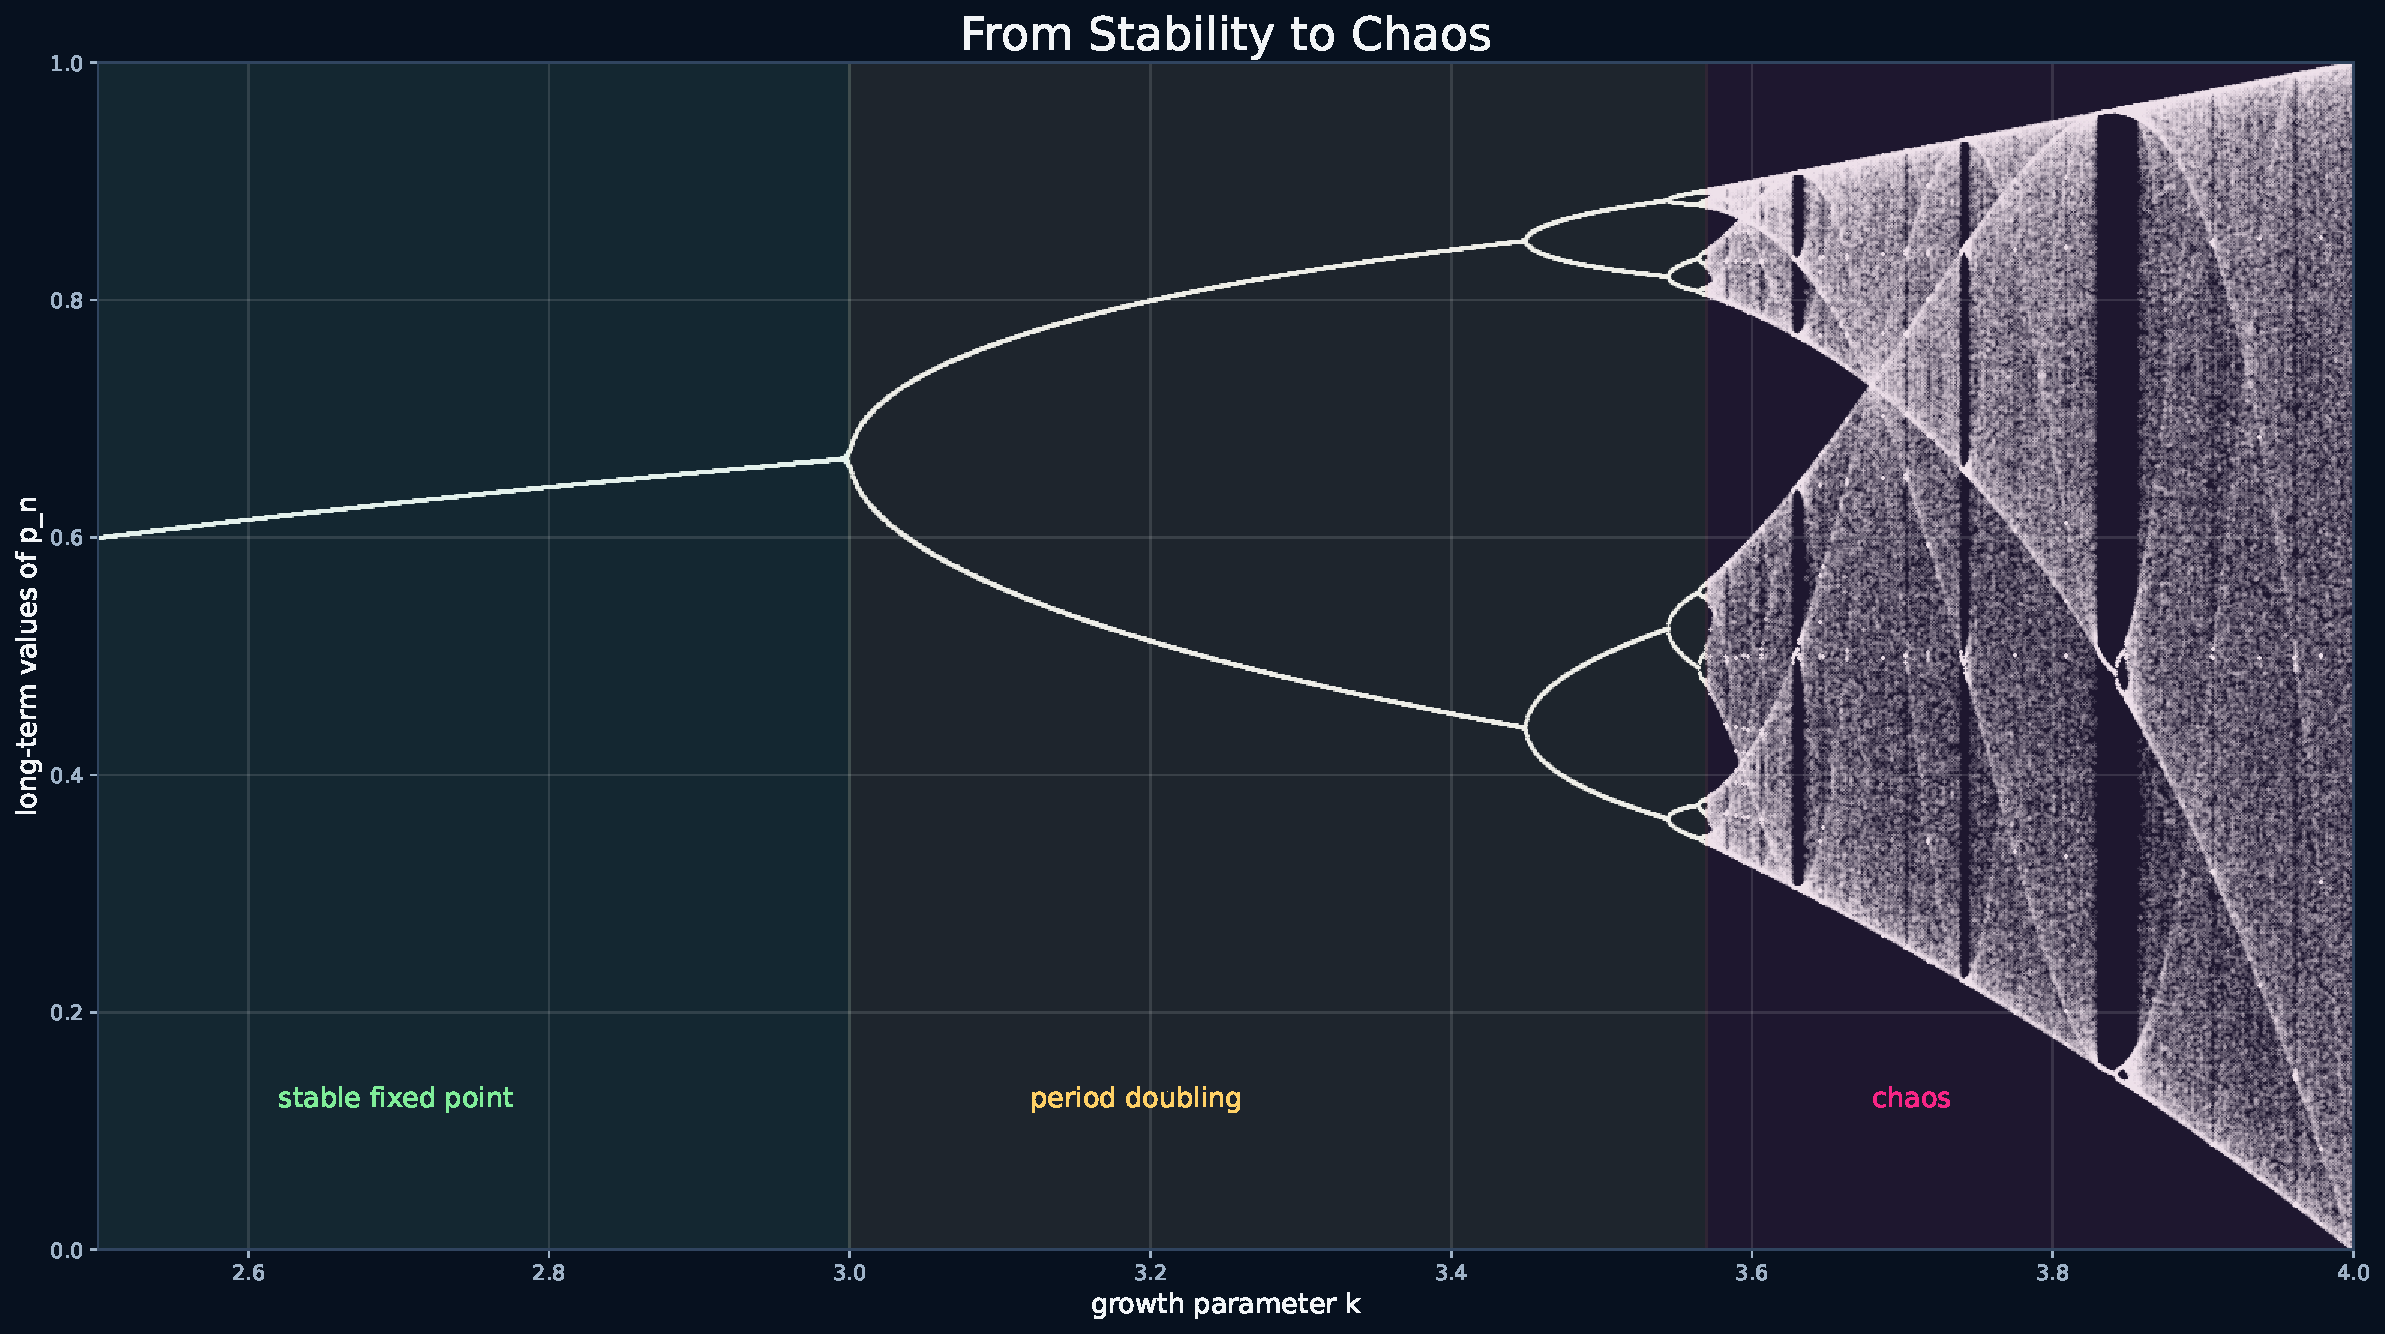
\includegraphics[width=\textwidth]{presentation_graphs/bifurcation_diagram_presentation.pdf}
\caption{Bifurcation diagram showing the transition from stability to chaos.}
\end{figure}

\begin{figure}[h!]
\centering
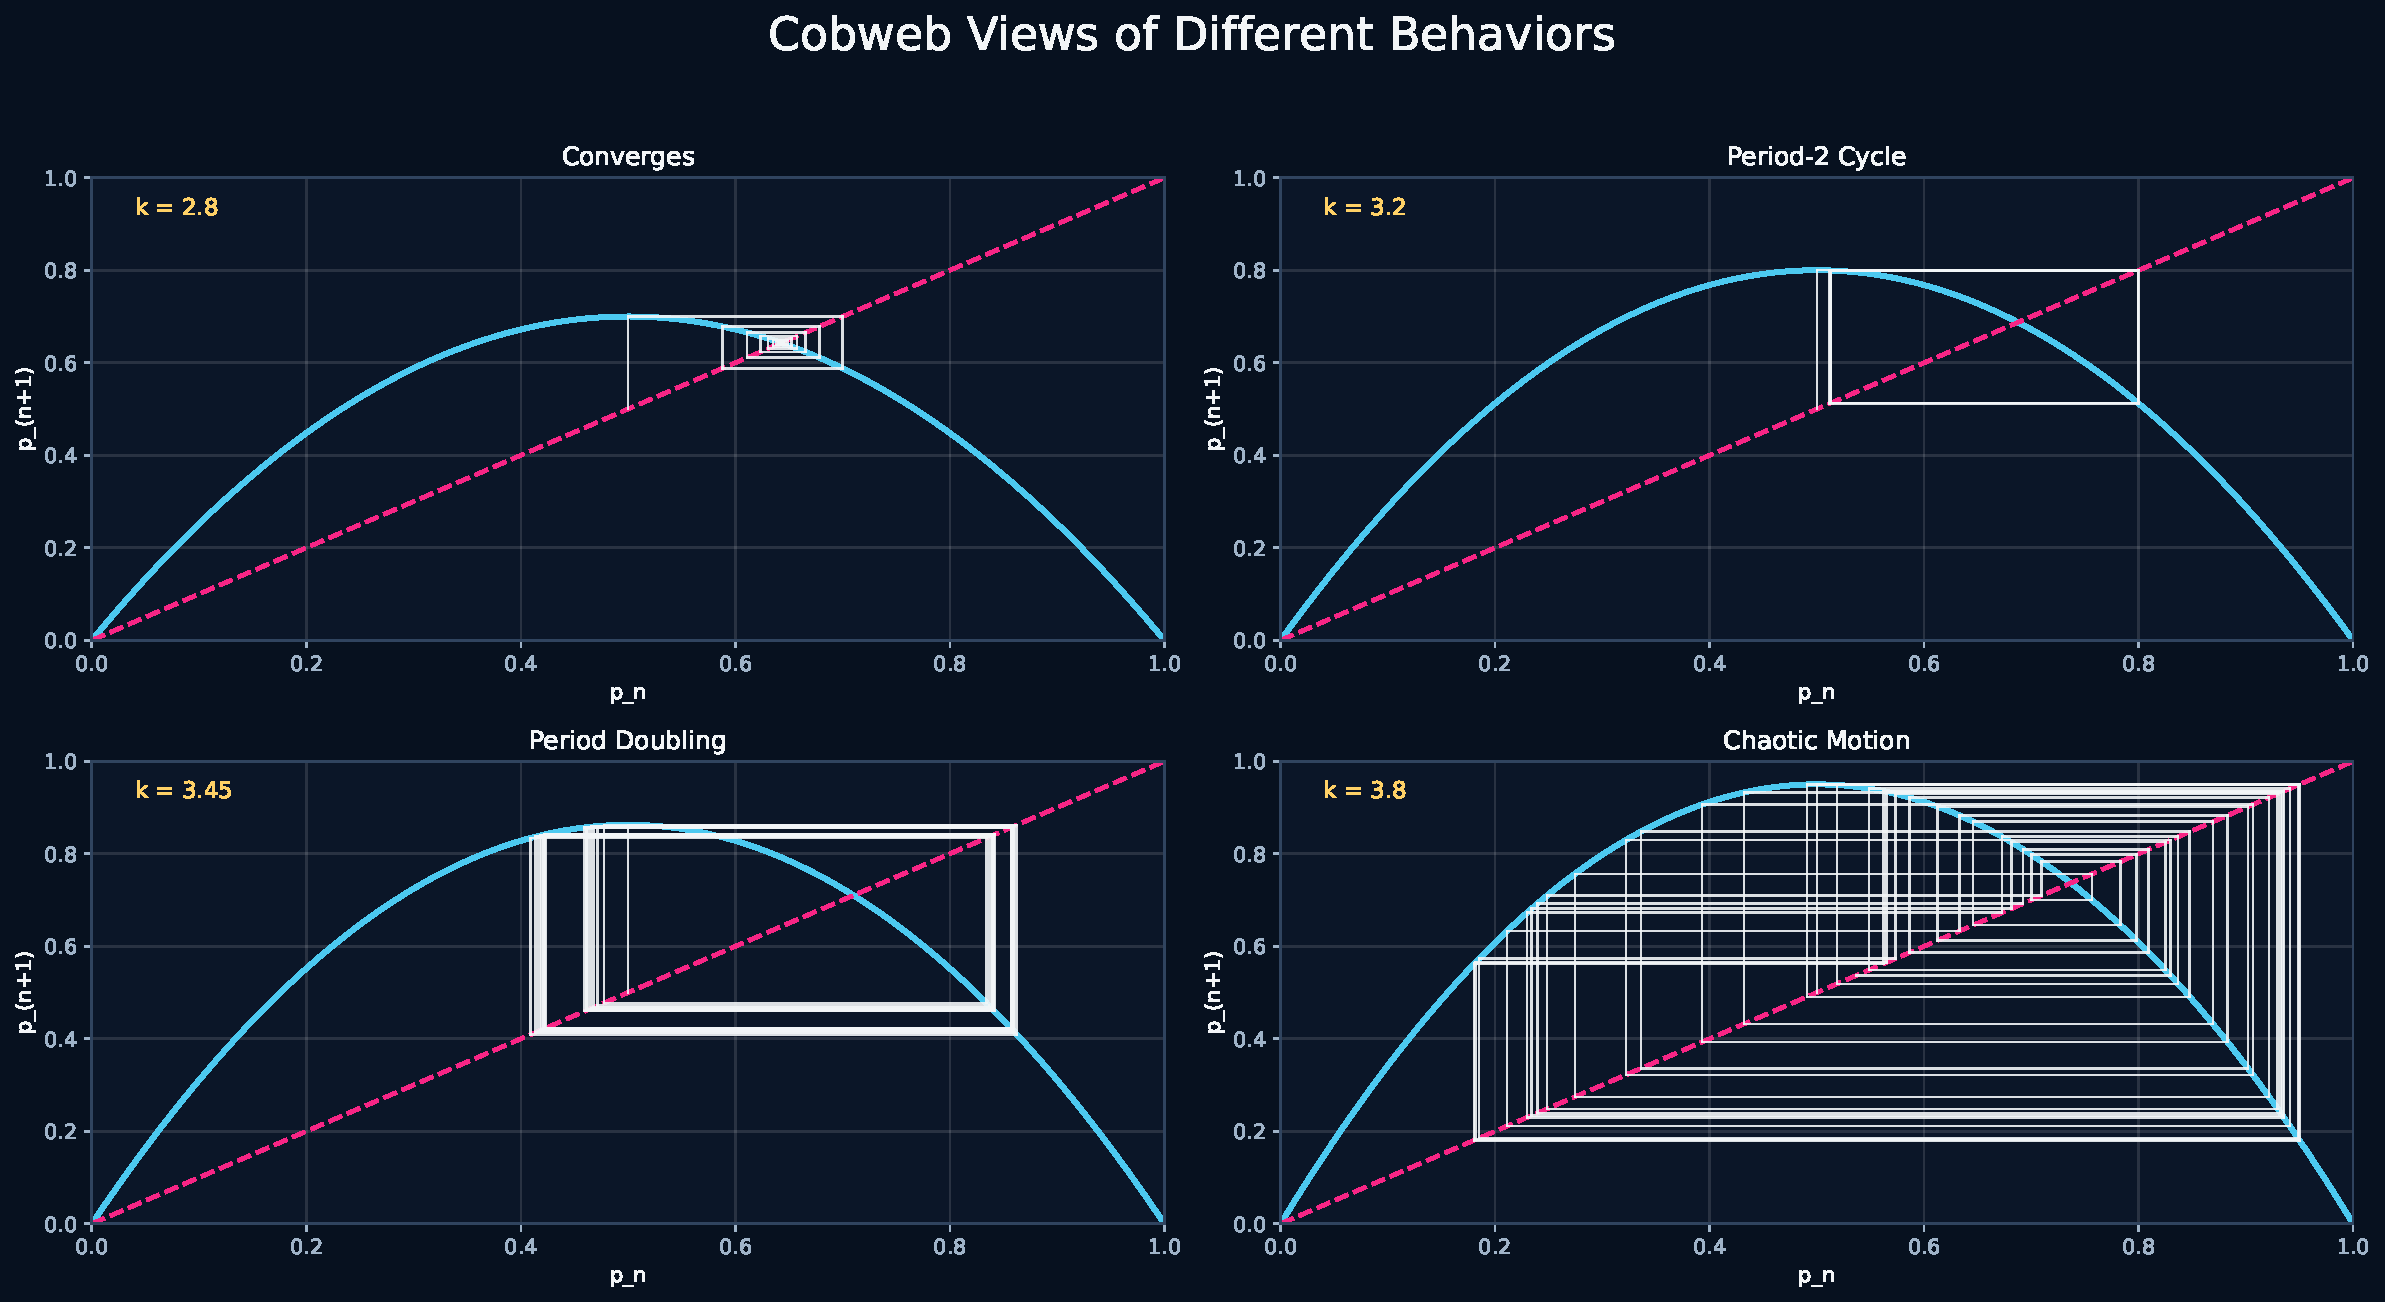
\includegraphics[width=\textwidth]{presentation_graphs/cobweb_grid.pdf}
\caption{Cobweb diagrams comparing convergence, cycles, period doubling, and chaos.}
\end{figure}

\begin{figure}[h!]
\centering
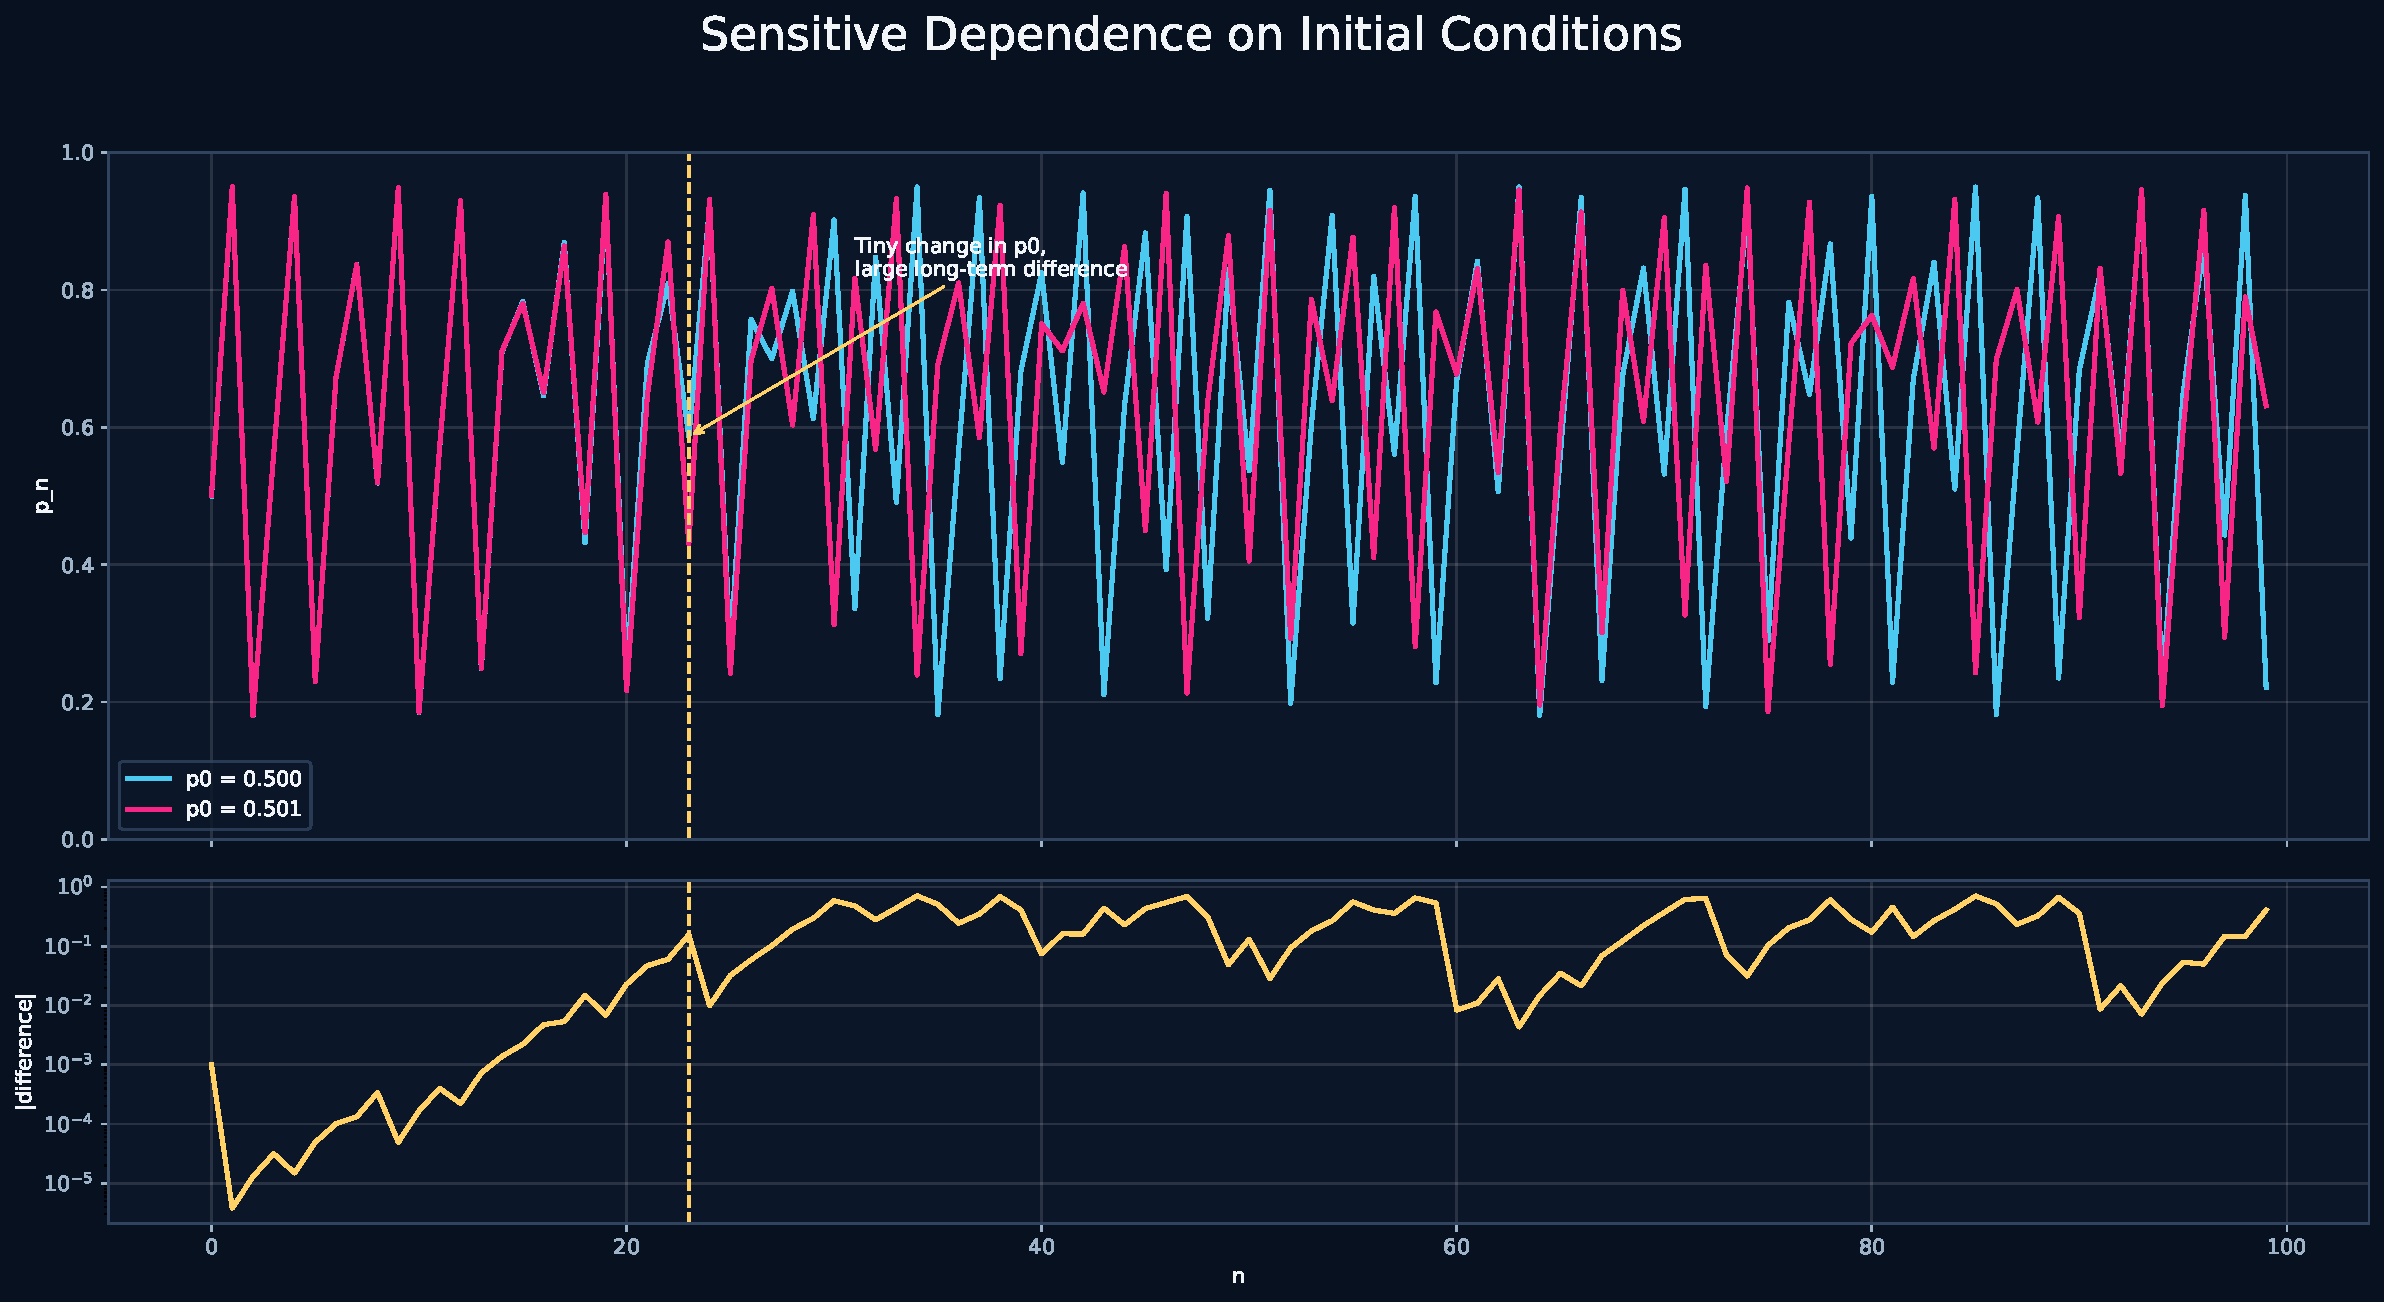
\includegraphics[width=\textwidth]{presentation_graphs/sensitivity_comparison.pdf}
\caption{Sensitivity to initial conditions for two very close starting values.}
\end{figure}

\begin{figure}[h!]
\centering
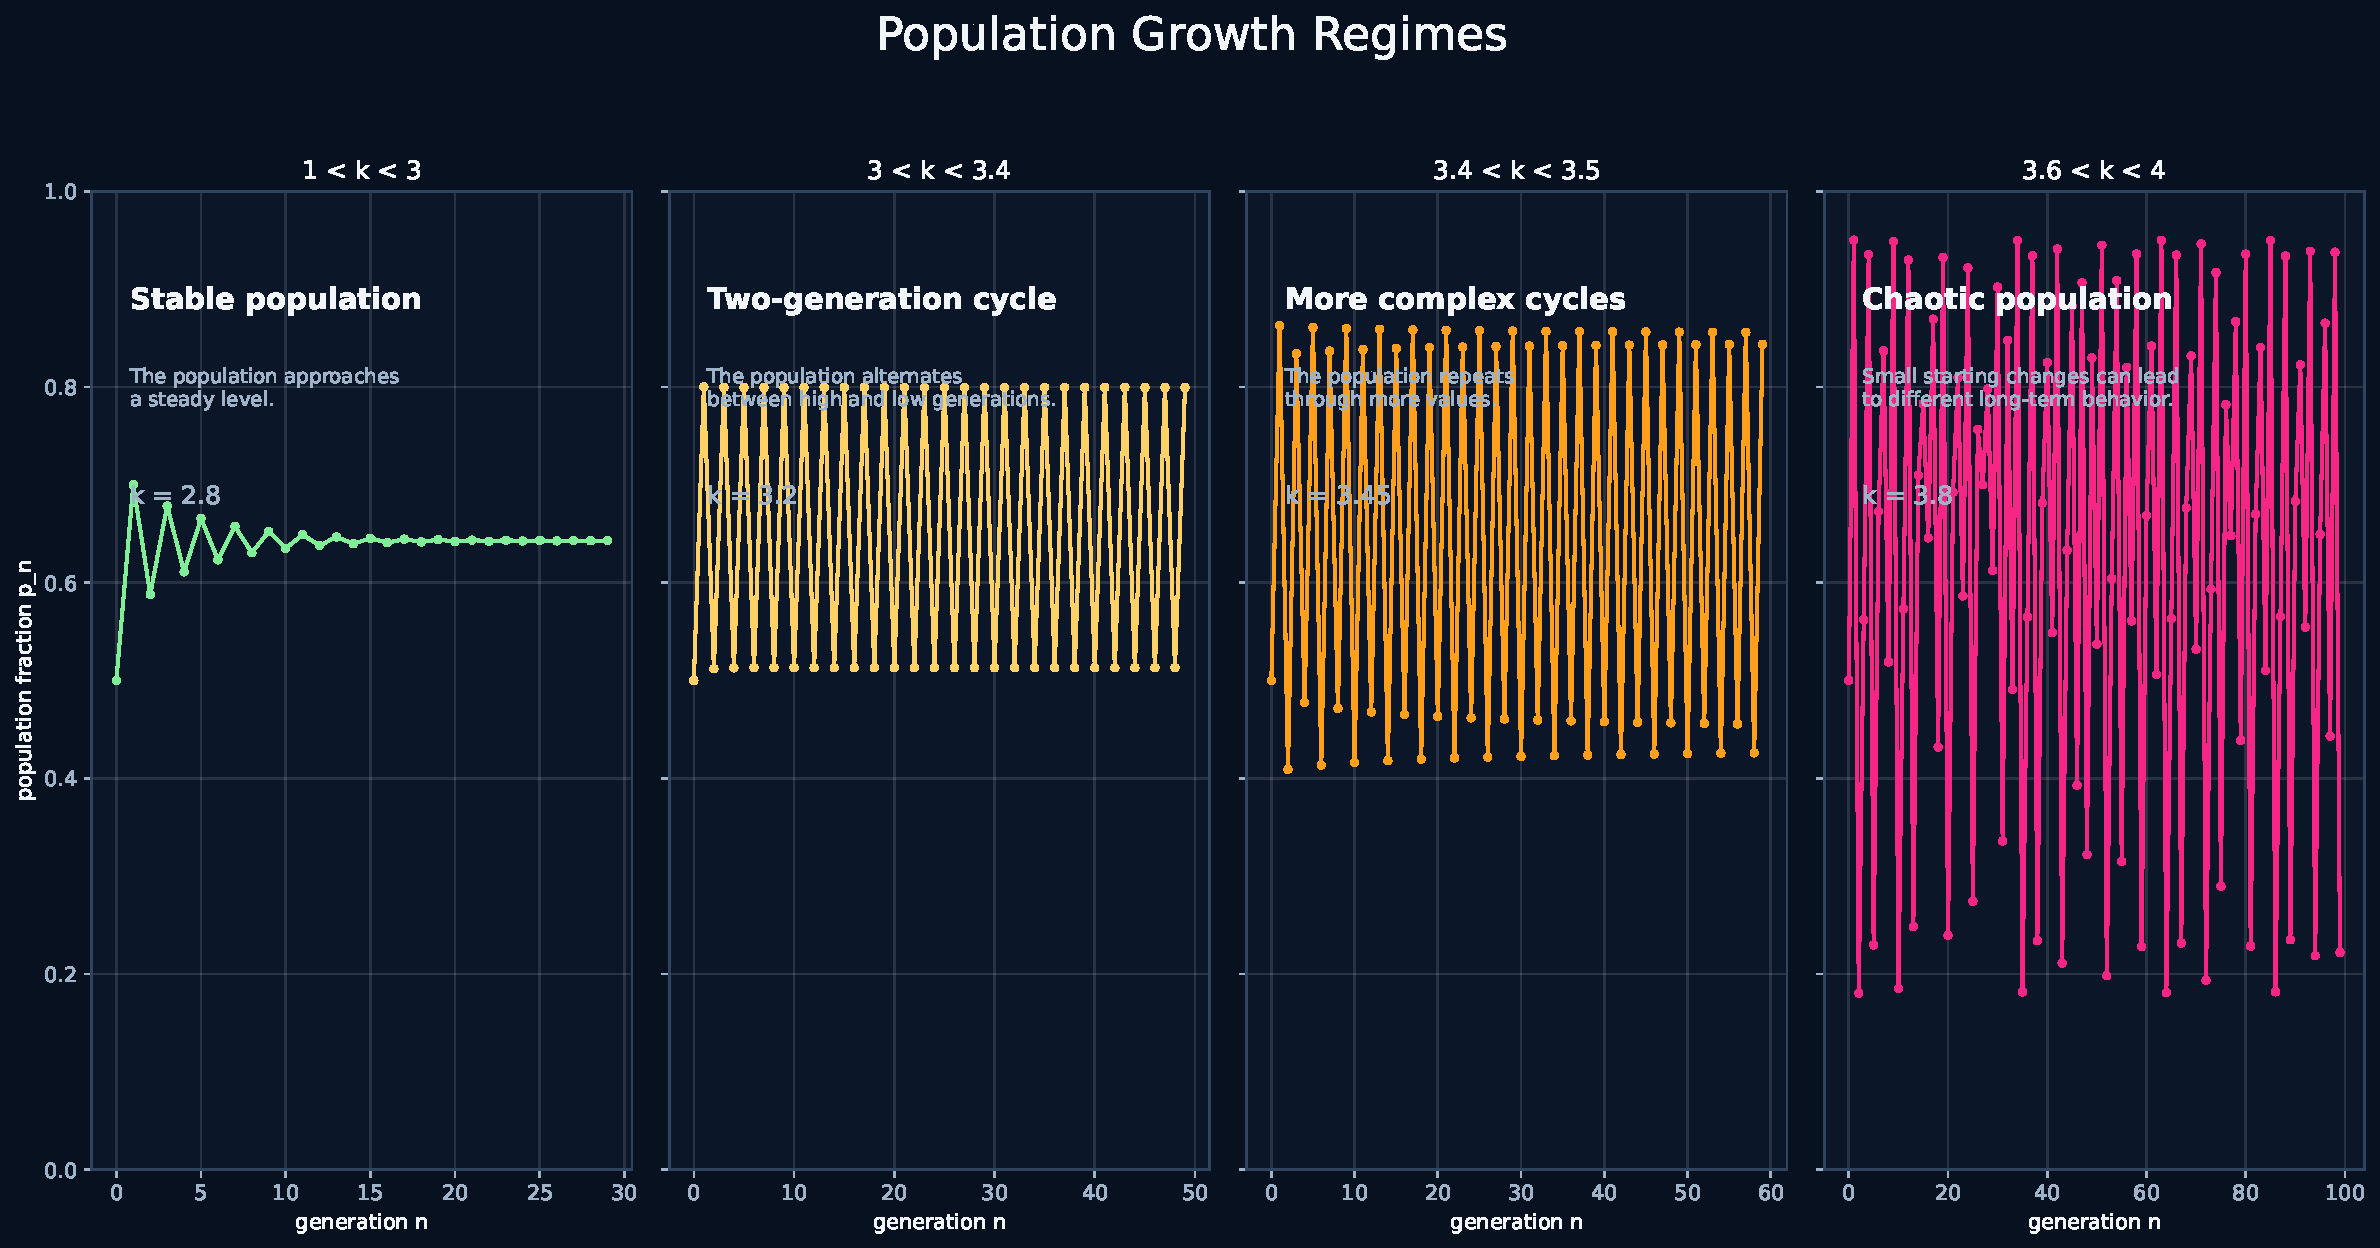
\includegraphics[width=\textwidth]{presentation_graphs/regime_summary.pdf}
\caption{Summary of the main behavior regimes of the logistic map.}
\end{figure}
